\documentclass[border=10pt]{standalone}
\usepackage{tikz}
\usetikzlibrary{arrows.meta}
\usepackage{xcolor}

% Brand colors
\definecolor{Garnet}{HTML}{73000A}
\definecolor{Atlantic}{HTML}{466A9F}
\definecolor{Congaree}{HTML}{1F414D}
\definecolor{Horseshoe}{HTML}{65780B}
\definecolor{Rose}{HTML}{CC2E40}
\definecolor{LightGray}{HTML}{ECECEC}

\begin{document}
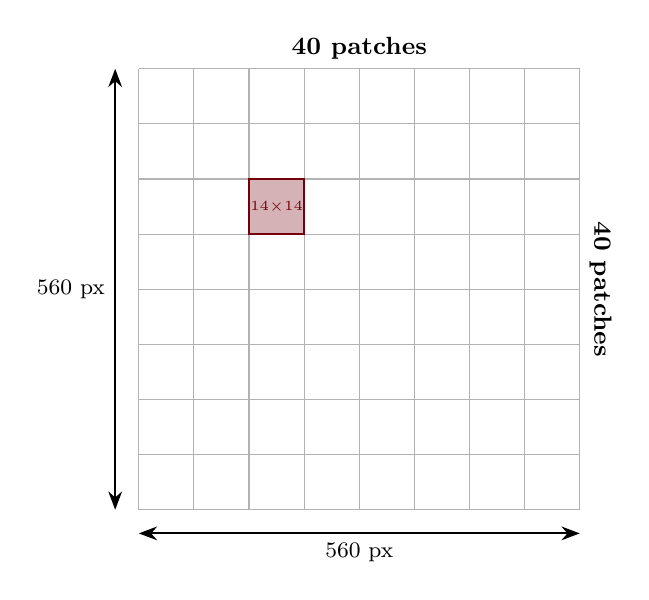
\begin{tikzpicture}[every node/.style={font=\small}]
\draw[step=0.7cm, black!30, thin] (0,0) grid (5.6,5.6);
\node[above] at (2.8, 5.6) {\textbf{40 patches}};
\node[rotate=270, above] at (5.6, 2.8) {\textbf{40 patches}};
\fill[Garnet!30] (1.4, 3.5) rectangle (2.1, 4.2);
\draw[Garnet, thick] (1.4, 3.5) rectangle (2.1, 4.2);
\node[font=\tiny, Garnet] at (1.75, 3.85) {$14{\times}14$};
\draw[{Stealth}-{Stealth}, thick] (-0.3, 0) -- (-0.3, 5.6) node[midway, left, font=\footnotesize] {560 px};
\draw[{Stealth}-{Stealth}, thick] (0, -0.3) -- (5.6, -0.3) node[midway, below, font=\footnotesize] {560 px};
\end{tikzpicture}
\end{document}
